% Created 2015-11-29 Вск 16:00
\documentclass[fleqn,12pt]{article}
\usepackage{euler}
\usepackage{amsmath}
\usepackage{epigraph}
\usepackage{mathtools}
\usepackage{amssymb}
\usepackage{proof}
\usepackage[pdftitle={Курс теории типов по Штукенбергу Д. Г.}]{hyperref}
\usepackage{amsthm}
\usepackage{stmaryrd} % ⟦⟧
\usepackage{enumitem} % 
\usepackage{xcolor} % red color for worries
\usepackage{pict2e} % templates
\usepackage[left=2cm,right=1.6cm,top=2cm,bottom=2cm,bindingoffset=0cm]{geometry}	
\usepackage{fontspec}
\setmainfont[Ligatures=TeX]{Palatino Linotype}
\setmonofont{DejaVu Sans Mono}
\usepackage{polyglossia}
\setdefaultlanguage[babelshorthands=true]{russian}

\renewcommand{\le}{\leqslant} % ≤
\renewcommand{\leq}{\leqslant} % ≤
\renewcommand{\ge}{\geqslant} % ≤
\renewcommand{\geq}{\geqslant} % ≤
\renewcommand{\phi}{\varphi}
\renewcommand{\epsilon}{\varepsilon}
\DeclareMathOperator{\plog}{plog}
\DeclareMathOperator{\Int}{Int}
\DeclareMathOperator{\Proof}{Proof}

\newcommand{\defeq}{\coloneqq}
\newcommand{\s}[1]{\texttt{#1}}
\newcommand{\xl}{$\lambda$}
\newcommand{\+}{\lambda}
\newcommand{\mbred}{$\ \longrightarrow\!\!\!\!\rightarrow_\beta\ $}
\newcommand{\lid}[1]{\textit{#1}}
\newcommand{\concat}{\hat{\ \ }}

\newcommand\myworries[1]{\textcolor{red}{#1}}

\def\ra{\rightarrow}

\renewcommand{\theenumii}{\asbuk{enumii}}
\AddEnumerateCounter{\asbuk}{\@asbuk}{ы}

\author{Daniyar Itegulov}
\date{\today}
\title{Курс теории типов по Штукенбергу Д.Г.}

\begin{document}
\theoremstyle{definition}
\newtheorem*{definition}{Определение}
\newtheorem*{example}{Пример}
\newtheorem{theorem}{Теорема}[section]
\newtheorem{axiom}{Аксиома}[section]
\newtheorem{lemma}[theorem]{Лемма}

\maketitle
\tableofcontents

\section{Предисловие и источники}
\label{sec-1}
\subsection{Предисловие}
\label{sec-1-1}
Я не отвечаю за верность написанного - много информации я придумал сам, много
достал из недостоверных источников.
\subsection{Источники}
\begin{enumerate}
  \item Лекции, данные напрямую Штукенбергом Д.Г.
  \item \href{https://github.com/shd/tt2014/blob/master/conspect.pdf}{Конспект Штукенберга Д.Г.}
  \item \href{http://disi.unitn.it/~bernardi/RSISE11/Papers/curry-howard.pdf}{Sørensen, Urzyczyn. Lectures on the Curry-Howard Isomorphism}
  \item \href{http://www.compsciclub.ru/csclub/sites/default/files/slides/20110313_systems_of_typed_lambda_calculi_moskvin_lecture06.pdf}{ПОМИ РАН презентация}
  \item \href{http://www.nsl.com/misc/papers/martelli-montanari.pdf}{Efficient unification algorithm}
  \item \href{http://starling.rinet.ru/~goga/tapl/tapl.pdf}{Пирс. Типы в языках программирования.}
  \item \href{http://math.nsc.ru/~asm256/lambda/LambdaDec2012.pdf}{Денотационная семантика Лямбда-исчисления}
  \item \href{http://r.duckduckgo.com/l/?kh=-1\&uddg=http://homepages.inf.ed.ac.uk/wadler/papers/lineartaste/lineartaste-revised.pdf}{The taste of linear logic}
  \item \href{http://plato.stanford.edu/entries/logic-linear/}{Stanford encyclopedia -- linear logic}
  \item \href{http://webdoc.sub.gwdg.de/ebook/serien/ah/UU-CS/2002-031.pdf}{Generalizing Hindley-Milner Type Inference Algorithms}
  \item \href{http://gallium.inria.fr/~fpottier/publis/emlti-final.pdf}{The essence of ML type inference (for H-M constraints)}
\end{enumerate}
\section{Ticket 1: Нетипизированное лямбда исчисление, теорема Чёрча-Россера}
\label{sec-2}
\subsection{Основные определения}
\label{sec-2-1}
\begin{eqnarray*}
$Variable = {v_0, v_1, v_2 \dots}$
\end{eqnarray*}
$Variable$ --- набор свободных переменных.
\begin{eqnarray*}
\Lambda^- &::=& Variable |
(\Lambda^- \Lambda^-) |
(\lambda Variable . \Lambda^-)
\end{eqnarray*}
$\Lambda^-$ --- пред-терм.
Конструкторы для пред-термов называются:
``Переменная'', ``Применение'' и ``Абстракция'' соответственно. \\
Ассоциативность пробела левая и тело абстракции имеет высший приоритет
(жадно набирает пока может).
\begin{example}
$\lambda x . a b c d e = \lambda x . ((((a b) c) d) e)$
\end{example}
Также допустимо писать $\lambda a b . A$ и это будет значить
$\lambda a . \lambda b . A$ (просто такой синтаксический сахар).

\begin{definition}
Определим функцию $freeVariables :: \Lambda^- \to [Variable]$. \\
Она будет находить все свободные переменные в пред-терме. \\
Более формально:
\begin{itemize}
\item $freeVariables(x) = \left\{x\right\}$
\item $freeVariables(A B) = freeVariables(A) \cup freeVariables(B)$
\item $freeVariables(\lambda x . A) = freeVariables(A) \setminus \left\{x\right\}$
\end{itemize}
Если $freeVariables(term) = \varnothing$, то терм $term$ называется замкнутым или
закрытым.
\end{definition}
\begin{definition}
Введём понятие ``подстановка''.
Будем обозначать $term[var:=otherTerm]$, если требуется в пред-терме $term$
подставить $otherTerm$ вместо всех свободных вхождений $var$. \\
Более формально:
\begin{itemize}
\item $x[x:=N] = N$
\item $y[x:=N] = y$
\item $(P Q)[x:=N] = P[x:=N] Q[x:=N]$
\item $(\lambda x . P)[x:=N] = \lambda x . P$
\item $(\lambda y . P)[x:=N] = \lambda z . P[y:=z][x:=N]$ если $y \in freeVariables(N)$
\item $(\lambda y . P)[x:=N] = \lambda y . P[x:=N]$ иначе
\end{itemize}
\end{definition}
\subsection{$\alpha$-эквивалентность и $\lambda$-термы}
\label{sec-2-2}
\begin{definition}
$\alpha$-эвивалентность ($=_\alpha$) -- наименьшее отношение на $\Lambda^-$,
что:
\begin{itemize}
\item $P =_\alpha P$ $\forall P$
\item $\lambda x . P =_\alpha \lambda y . P [x:=y]$ если $y \not \in freeVariables(P)$
\end{itemize}
Также введём следующую операцию: $[M]_\alpha = \left\{ N \in \Lambda^- | M =_\alpha N \right\}$
\end{definition}
\begin{definition}
$\Lambda = \Lambda^-_{=_\alpha} = \left\{ [M]_\alpha | M \in \Lambda^- \right\}$
\end{definition}
Отсюда и дальше под термами мы будем подразумевать лямбда-термы, а не 
пред-термы, если не написано иначе.
\begin{definition}
Свободные переменные у лямбда-термов определяются точно так же
как и у пред-термов
\end{definition}
\begin{definition}
Подстановка в лямбда-термы определяются точно так же за исключением
подстановки в применение: \\
$(\lambda y . P)[x:=N] = \lambda y . P[x:= N]$, если $x \not= y$,
где $y \not \in freeVariables(N)$
\end{definition}

\section{Ticket 2: Булевские значения, чёрчевские нумералы, упорядоченные пары,
  алгебраические типы. Нормальный и аппликативный порядок редукции.
  Бета-эквивалентность и Y-комбинатор. Парадокс Карри.}
\label{sec-3}
\subsection{Булевские значения}
\label{sec-3-1}
Значения Булевской логики можно определить так:

\begin{align*}
T &= \lambda x . \lambda y . x \\
F &= \lambda x . \lambda y . y
\end{align*}

Очевидно это просто два проектора. Определим несколько интересных операций в
булевской логике:

\begin{align*}
ifThenElse &= \lambda A . \lambda P . \lambda Q . A P Q \\
and &= \lambda A . \lambda B . A B F \\
not &= \lambda A . A F T \\
xor &= \lambda A . \lambda B . A (not B) B
\end{align*}

\subsection{Пары}
\label{sec-3-2}
Пара и её проекторы определяются следующим образом:
\begin{align*}
\langle A, B \rangle &= \lambda x . x A B \\
\pi_1 &= \lambda x . \lambda y . x \\
\pi_2 &= \lambda x . \lambda y . y \\
fst &= \lambda p . p \pi_1 \\
snd &= \lambda p . p \pi_2
\end{align*}

\subsection{Чёрчевские нумералы}
\label{sec-3-3}

Определим $n$-разовое приминение функции $f$ как:
\begin{align*}
f^0(A) &= A \\
f^{n+1}(A) &= f(f^n(A))
\end{align*}

Тогда пусть $\bar{n}$ будет $n$-ым Чёрчевским нумералом, если:
\begin{equation}
\bar{n} = \lambda f . \lambda x . f^n(x)
\end{equation}

Наблюдение: $\bar{0} = F$.

Определим арифметику на Чёрчевских нумералах:
\begin{align*}
isZero &= \lambda a . a \lambda x . F) T \\
inc &= \lambda a . \lambda f . \lambda x . f (a f x) \\
plus &= \lambda a . \lambda  b . \lambda f . \lambda x . a f (b f x) \\
mul &= \lambda a . \lambda b . \lambda f . a (b f) \\
pow &= \lambda a . \lambda b . b a
\end{align*}

Понимать их следует так: $isZero$ значит, что если хоть раз будет применено $f$, 
то число не ноль, иначе ноль. $inc$ значит, что нужно ещё
один раз применить $f$ к $a$. $plus$ значит, что нужно просто передать значение
$a$ как начальное значение $b$.

Также с помощью пар можно реализовать вычитание. Начнём с $\langle 0, 0 \rangle$ и будем
поддерживать пару $\langle n, n - 1 \rangle$, пока $n$ не окажется равным $a$.
\begin{equation}
dec = \lambda a . snd (a (\lambda p . \langle inc (fst p); fst p \rangle ) \langle 0, 0 \rangle )
\end{equation}

\subsection{Алгебраические типы}
\label{sec-3-4}

\myworries{Алгебраический тип -- любой сложный тип, состоящий из более простых
  типов}

\subsection{Нормальный и аппликативный порядок редукции}
\label{sec-3-5}
Рассмотрим способы редуцирования терма
\begin{align*}
v &\not\rightarrow_\beta \\
\lambda x . M &\rightarrow_\beta \lambda x . M' \\
M N &\rightarrow_\beta M' N \\
M N &\rightarrow_\beta M N'
\end{align*}
Получается, что выбор в редуцировании возникает только в аппликации. Тогда
определим эти порядки редукции:

Нормальный порядок редукции -- редукция, при которой первым делом сокращается
редекс $(\lambda x . M) N$.

Аппликативный порядок редукции -- редукция, при которой первым делом сокращается
$N$, а затем уже редекс $(\lambda x . M) N'$.

\subsection{$\beta$-эквивалентность}
\label{sec-3-6}

Бинарное отношение $=_\beta$ над $\Lambda$ определяется индуктивно:

\begin{align*}
M \twoheadrightarrow_\beta N &\Rightarrow M =_\beta N \\
M =_\beta N &\Rightarrow N =_\beta M \\
M =_\beta N, N =_\beta L &\Rightarrow M =_\beta L
\end{align*}

Интуитивно: два терма $M$ и $N$ связаны отношением $=_\beta$, если есть
связывающая их цепочка $\rightarrow_\beta$-стрелок.

Пример: \\
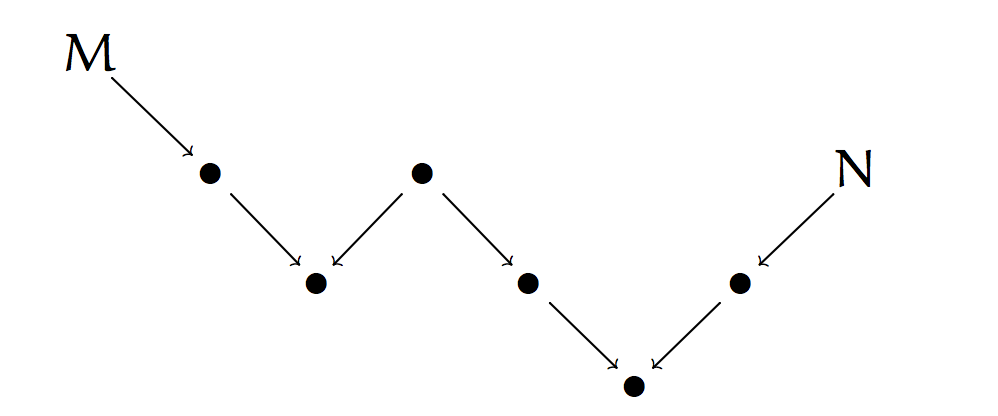
\includegraphics[scale=0.5]{resources/beta_equality.png}

\subsection{Y-комбинатор}
\label{sec-3-7}

\begin{theorem}
Для любого $F$ найдётся такой $X$ (неподвижная точка), что:
\begin{equation}
F X =_\beta X
\end{equation}
\end{theorem}
\begin{proof}
Пусть $W = \lambda x . F (x x)$, а $X = WW$. Тогда $X = WW = (\lambda x . F (x
x)) W = F (W W) = F X$
\end{proof}

\begin{theorem}
Существует комбинатор неподвижной точки $Y = \lambda f . (\lambda x . f (x x))
(\lambda x . f (x x))$ такой, что $\forall F \  F (Y F) = Y F$
\end{theorem}
\begin{proof}
Очевидно если расписать $Y F$
\end{proof}

% \myworries{Возможно стоит сказать о F =_\beta M[f:=F]}

\subsection{Парадокс Карри}

Построим исчисление высказываний на основе язык лямбда выражений. Для этого
добавим к аппликации импликацию ($\supset$), которое будет действовать по
следующим правилам:

\begin{align*}
A =_\beta B &\Rightarrow \ \vdash A \supset B \\
A =_\beta B &\Rightarrow \ \vdash B \supset A \\
\end{align*}

Также мы ожидаем доказуемости следующих свойств:

\begin{align*}
&\vdash \alpha \supset \alpha \\
\alpha \supset \alpha \supset \beta &\vdash \alpha \supset \beta 
\end{align*}

Однако, так построенное исчисление черезчур мощно, о чём свидетельствует
следующее утверждение:

Рассмотрим выражение $F_\alpha \equiv \lambda x. x x \supset \alpha$ 
и выражение $\Phi_\alpha \equiv F_\alpha F_\alpha$.
Нетрудно видеть, что $\Phi_\alpha =_\beta \Phi_\alpha \supset \alpha$.
Тогда: \\

\begin{tabular}{ll}
$\vdash \Phi_\alpha \supset \Phi_\alpha$ & Доказуемое утверждение\\
$\vdash \Phi_\alpha \supset \Phi_\alpha \supset \alpha$ & По определению ($=_\beta$)\\
$\vdash (\Phi_\alpha \supset \Phi_\alpha \supset \alpha) \supset (\Phi_\alpha \supset \alpha)$ & Доказуемое утверждение\\
$\vdash \Phi_\alpha \supset \alpha$ & M.P.\\
$\vdash \Phi_\alpha$ & бета-эквивалентность\\
$\vdash \alpha$ & M.P.
\end{tabular}

Таким образом мы показали, что любое утверждение может быть выведено в данной
системе, т.е. система противоречива.
\section{Ticket 3: Просто типизированное лямбда-исчисление. Исчисление по Чёрчу и по Карри.
Основные леммы, изоморфизм Карри-Ховарда. Нетипизируемость Y-комбинатора.}
\label{sec-4}
\subsection{Простотипизированное лямбда-исчисление по Карри}
\label{sec-4-1}
Пусть $U$ -- множество простых (атомарных) типов. \\
Грамматика для типов: $\Pi = U | \Pi \rightarrow \Pi$

Контекстом будем называть множество пар вида $x_n:\tau_n$, причем $x_i \not =
x_j$, для $i \not = j$.
\begin{align*}
dom(\Gamma) = \{ x_i | x_i:\tau_i \in \Gamma \} \\
range(\Gamma) = \{ \tau_i | x_i:\tau_i in \Gamma \}
\end{align*}

Аксиомы типизации:

\begin{enumerate}
\item
$\infer{\Gamma, x:\tau \vdash x:\tau}{}$
\item
$\infer{\Gamma \vdash (M N):\tau}{\Gamma \vdash M: \sigma \rightarrow
\tau; \Gamma \vdash N: \sigma}$
\item
$\infer{\Gamma \vdash \lambda x. M: \sigma \rightarrow \tau}{\Gamma, x:\sigma \vdash M:\tau}$
\end{enumerate}

$M \in \Lambda$ называется типизируемым, если существуют $\Gamma$ и $\sigma$
такие, что $\Gamma \vdash M:\sigma$. Таким образом будем называть простотипизированным лямбда-исчислением тройку
$(\Lambda, \Pi, \vdash)$.

Определим подстановку типа $\tau$ вместо $\alpha$ в тип $\sigma$
($\sigma[\alpha:=\tau]$):
\begin{align*}
\alpha[\alpha:=\tau] &= \tau \\
\beta[\alpha:=\tau] &= \beta \\
(\sigma_1 \rightarrow \sigma_2)[\alpha:=\tau] &= \sigma_1[\alpha:=\tau] \rightarrow \sigma_2[\alpha:=\tau]
\end{align*}

Нотация $\Gamma[\alpha:=\tau]$ обозначает $\{ (x:\sigma[\alpha:=\tau] |
(x:\sigma) \in \Gamma) \}$

\subsection{Базовые леммы}
\label{sec-4-2}

\myworries{TODO: Тут надо расписать не очень интеллектуальные и не очень интересные
  леммы}

\subsection{Нетипизируемость Y-комбинатора}
\label{sec-4-3}

Запихиваем $(\lambda x . x x) (\lambda x . x x)$ в type-inference алгоритм и он
скажет, что типа нет.

\myworries{TODO: Тут надо написать что-то более формальное и если у кого-то есть
свободное время, то прошу}


\subsection{Простотипизированное лямбда-исчисление по Чёрчу}
\label{sec-4-3}

Пусть $V_\sigma$ -- набор свободных переменных типа $\sigma$. Тогда:
\begin{align*}
x \in V_\sigma &\Rightarrow x \in \Lambda_\sigma \\
M \in \Lambda_{\sigma \rightarrow \tau}; N \in \Lambda_{\sigma} &\Rightarrow M N \in \Lambda_\tau \\
M \in \Lambda_\tau; x \in \Lambda_\sigma &\Rightarrow \lambda x^\sigma . M \in \Lambda_{\sigma \rightarrow \tau}
\end{align*}
Псевдо-терм: $\Lambda_\pi := V | (\lambda x:\Pi: \Lambda_\pi) | (\Lambda_\pi
\Lambda_\pi)$
\end{document}
% Local Variables:
% TeX-engine: xetex
% End:
